\subsection{Armour}

\begin{table*}[!htb]
\begin{GenesysTable}{Armour}{armour}{ =l +l +l +l +l +l +l +X}
Name                                    & Defense   & Soak  & Encum & Price     & Rarity    & HP    & Special  \\
\nameref{itmamr:heavyrobes}             & 1         & +0    & 1     & 5cp       & 1         & 1     & \\
%\nameref{itmamr:padded}                 & 1         & +0    & 1     & 5cp       & 1         & 1     & \\
\nameref{itmamr:crodluleather}          & 0         & +1    & 2     & 10cp      & 1         & 1     & \iqtyref{fragile} \\
%\nameref{itmamr:baazragleather}         & 0         & +1    & 2     & 10cp      & 1         & 1     & \iqtyref{fragile} \\
\nameref{itmamr:kankhide}               & 1         & +1    & 2     & 25cp      & 3         & 1     & \iqtyref{fragile} \\
%\nameref{itmamr:brohghide}              & 1         & +1    & 2     & 25cp      & 3         & 1     & \iqtyref{fragile} \\
\nameref{itmamr:reaperchitin}           & 0         & +2    & 3     & 50cp      & 4         & 2     & \iqtyref{fragile}, \iqtyref{solid} 1 \\
%\nameref{itmamr:kreenchitin}            & 0         & +2    & 3     & 50cp      & 4         & 1     & \iqtyref{fragile}, \iqtyref{solid} 1 \\
\nameref{itmamr:anakoreshell}           & 1         & +2    & 3     & 100cp     & 5         & 1     & \iqtyref{fragile}, \iqtyref{noisy}, \iqtyref{solid} 2 \\
%\nameref{itmamr:inixshell}              & 1         & +2    & 3     & 100cp     & 5         & 3     & \iqtyref{fragile}, \iqtyref{noisy}, \iqtyref{solid} 2 \\
\nameref{itmamr:braxatbreastplate}      & 1         & +2    & 3     & 200cp     & 6         & 1     & \iqtyref{fragile}\\
\nameref{itmamr:braxathalfplate}        & 2         & +3    & 4     & 1000cp    & 7         & 2     & \iqtyref{fragile}, \iqtyref{restrictive}, \iqtyref{solid} 2 \\
\nameref{itmamr:braxatfullplate}        & 3         & +3    & 5     & 2000cp    & 8         & 2     & \iqtyref{fragile}, \iqtyref{restrictive}, \iqtyref{solid} 3 \\
\nameref{itmamr:mekillotbreastplate}    & 1         & +2    & 3     & 1500cp    & 6         & 2     & \iqtyref{noisy},   \iqtyref{reinforced}\\
\nameref{itmamr:mekillothalfplate}      & 1         & +3    & 4     & 3000cp    & 7         & 2     & \iqtyref{noisy},   \iqtyref{reinforced}, \iqtyref{solid} 2 \\
\nameref{itmamr:mekillotfullplate}      & 2         & +3    & 5     & 5000cp    & 8         & 2     & \iqtyref{noisy},   \iqtyref{reinforced}, \iqtyref{solid} 3 \\
\end{GenesysTable}
\end{table*}

\begin{figure}[!htb]
\centering
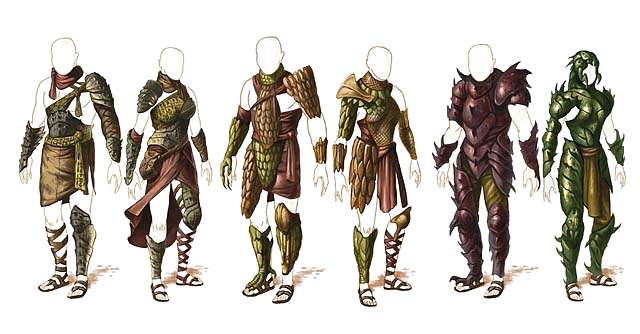
\includegraphics[width=0.5\linewidth]{images/athasian_armour.png}
\end{figure}

\FloatBarrier

\begin{multicols}{2}

\subsubsection{Heavy Robes}
\label{itmamr:heavyrobes}
These are robes made of multiple layers of thick robe.

%\subsubsection{Padded Armour}
%\label{itmamr:padded}
%Padded armour is made of heavy cloth and batting. Many Athasian warriors prefer padded armour woven from giant hair.

\subsubsection{Crodlu Leather}
\label{itmamr:crodluleather}
This armour is crafted using hardened leather from Crodlu reinforced with bone and talons.

%\subsubsection{Baazrag Leather}
%\label{itmamr:baazragleather}
%This armour is crafted using the hardened underhide from Baazrag combined with the cheaper parts of their shell.

\subsubsection{Kank Hide Armour}
\label{itmamr:kankhide}
This armour is skillfully made by interlocking hexagonal bits of a kank’s carapace.

\subsubsection{Brohg Hide Armour}
\label{itmamr:brohghide}
This armour is made from the hardened hide from a Brogh.

\subsubsection{Reaper Chitin Armour}
\label{itmamr:reaperchitin}
This chitin armour is made from the hard chitin from a Dune Reaper.

%\subsubsection{Kank Chitin Armour}
%\label{itmamr:kreenchitin}
%Thi chiitin armour is made from insect shell of a Kank.

\subsubsection{Anakore Shell Armour}
\label{itmamr:anakoreshell}
This shell armour made from interlocking shells from an Anakore, combined with the hardened leather of the underhide and their bones.

%\subsubsection{Inix Shell Armour}
%\label{itmamr:inixshell}
%This shell armour is made by weaving giant's hair around the breast shells from Inix'.

\subsubsection{Braxat Breastplate}
\label{itmamr:braxatbreastplate}
These armours are constructed using choice plates taken from Braxat.

\subsubsection{Mekillot Breastplate}
\label{itmamr:mekillotbreastplate}
These armours are constructed using choice plates taken Mekillot.

\subsubsection{Braxat Half Plate}
\label{itmamr:braxathalfplate}
These armours are constructed using choice plates taken from Braxat.

\subsubsection{Mekillot Half Plate}
\label{itmamr:mekillothalfplate}
These armours are constructed using choice plates taken Mekillot.

\subsubsection{Braxat Full Plate}
\label{itmamr:braxatfullplate}
These armours are constructed using choice plates taken from Braxat.

\subsubsection{Mekillot Full Plate}
\label{itmamr:mekillotfullplate}
These armours are constructed using choice plates taken Mekillot.

\end{multicols}
